
\subsection{Relaciones y funciones}

\subsubsection{Pares ordenados}

Un par ordenado es aquel en el cual el \textit{orden} de los elementos tiene importancia. Es decir, es aquel donde 
\(A = \{a , b\} \neq  A = \{b , a\}\), excepto sí \(a = b\). Los pares, ternas, cuadruplas ordenadas 
de elementos se pueden llamar en forma colectiva \textit{conjuntos ordenados}, y estos se encierran entre paréntesis 
y no entre llaves, es decir que cuando queremos denotar que un conjunto es ordenado se haria así \(A = (a , b)\)

\begin{ejemplo}
    Los pares ordenados serian utiles para mostrar la edad y el peso de cada estudiante de una clase, se pueden formar 
    pares ordenados de \((edad , peso)\). Podemos ver que \((19 , 127)\) y  \((127 , 19)\) obviamente
    indican cosa diferentes.
\end{ejemplo}

En un plano coordenado rectangular (cartesiano), donde el eje \(x\) y el eje \(y\) se cruzan entre si en un angulo 
recto, dividiendo el plano en cuatro cuadrantes. El plano \(x \, y\) es un conjunto infinitos de puntos, cada
punto representa un par ordenado donde el primer elemento es \(x\) y el segundo elemento es \(y\). Por lo tanto 
un el punto \((4 , 2)\) es \(\neq\) que el punto \((2 , 4)\). Esto se puede observar en la figura \ref{cuadro_cartesiano}.

\begin{figure}[!ht]
    \centering
    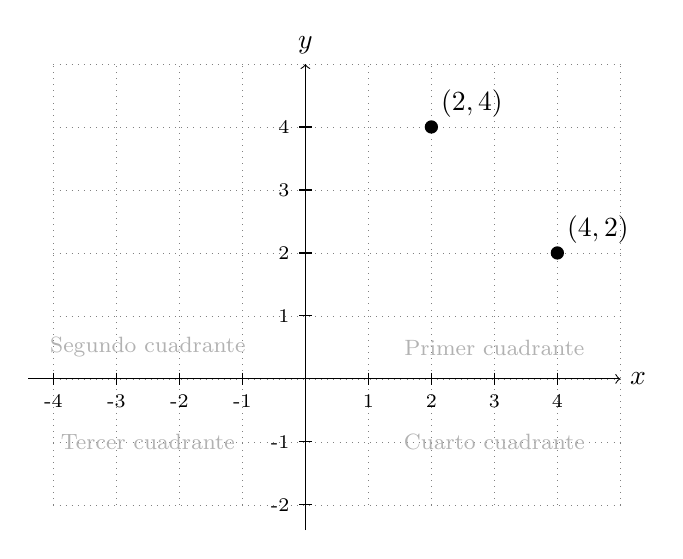
\begin{tikzpicture}[scale=0.8]

        % Cuadrícula suave
        \draw[step=1cm, gray, very thin, dotted] (-4,-2) grid (5,5);
        
        % Ejes
        \draw[->] (-4.4,0) -- (5,0) node[right] {$x$};
        \draw[->] (0,-2.4) -- (0,5) node[above] {$y$};
        
        % Marcas y números eje x
        \foreach \x in {-4,-3,-2,-1,1,2,3,4}
            \draw (\x,0.1) -- (\x,-0.1) node[below] {\scriptsize \x};
        
        % Marcas y números eje y
        \foreach \y in {-2,-1,1,2,3,4}
            \draw (0.1,\y) -- (-0.1,\y) node[left] {\scriptsize \y};
        
        % Punto (4,2)
        \fill (4,2) circle (3pt);
        \node[above right] at (4,2) {$(4,2)$};
        
        % Punto (2,4)
        \fill (2,4) circle (3pt);
        \node[above right] at (2,4) {$(2,4)$};
        
        % Nombre de los cuadrantes
        \node[gray!60] at (3,0.5) {\footnotesize Primer cuadrante};
        \node[gray!60] at (-2.5,0.5) {\footnotesize Segundo cuadrante};
        \node[gray!60] at (-2.5,-1) {\footnotesize Tercer cuadrante};
        \node[gray!60] at (3,-1) {\footnotesize Cuarto cuadrante};
    
    \end{tikzpicture}
    \caption{Cuadro cartesiano con sus respectivos puntos \((4 , 2)\) y \((2 , 4)\)}
    \label{cuadro_cartesiano}
\end{figure}



El \textit{producto cartesiano} o \textit{producto directo} es aquel en el cual a partir de dos conjuntos específicos \(x = \{1,2\}\) y \(y = \{3,4\}\), se desea formar \textit{pares ordenados} utilizando los elementos del primer conjunto y los del segundo conjunto. El resultado serian cuatro pares ordenados \((1,3),(1,4),(2,3),(2,4)\).

El \textit{producto cartesiano} se denota mediante \(\times\), la cual se lee como ``cruz''. Por lo tanto siguiendo el producto cartesiano anterior, este se denotaria como \(x\times y\). Por lo tanto este producto se va a expresar como 
\[
x \times y = \{(1,3),(1,4),(2,3),(2,4)\}
\]
Aplicando lo anterior, se puede tomar como la definicion general del producto cartesiano, para cualquiera de los conjuntos dados \(x \times y\) como 
\[
x \times y = \{(a,b) | a \in x \quad \text{y} \quad b \in y\}
\]
Si ahora se permite que \(x\) y \(y\) incluyan los números reales, entonces el producto cartesiano resultante seria
\[
x \times y = \{(a,b) | a \in \mathbb{R} \quad \text{y} \quad b \in \mathbb{R}\}
\]

Cada par ordenado corresponde a un punto \textit{único} en el plano coordenado cartesiano, y por lo tanto cada punto del plano coordenado también corresponde a un par ordenado \textit{único} en el conjunto \(x \times y\). El punto \(x \times y\) es el lugar donde se cruza el eje \(x\) y el eje \(y\). 

Tambien podriamos definir el producto cartesiano de tres conjuntos \(x\), \(y\) y \(z\) de la siguiente manera
\[
x \times y \times z = \{(a,b,c) | a \in x , b \in y , c \in z\}
\]

Si los conjuntos \(x\), \(y\) y \(z\) constan de números reales, el producto cartesiano corresponder á al conjunto de los puntos en un espacio tridimensional. Esto se puede denotar como \(\mathbb{R} \times \mathbb{R} \times \mathbb{R}\), o de forma concisa \(\mathbb{R}^3\).


\subsubsection{Relaciones y funciones}

Todo subconjunto de un producto cartesiano construye una relación entre \(y\) y \(x\). Por conveniencia los elementos de \(x \times y\) se escribira como \(x,y\), por lo tanto ahora \(x\) e \(y\) son variables.

\begin{ejemplo}
    \label{ejemplo_1.1.2}
    El conjunto \(\{(x,y)|y=2x\}\) es un conjunto de pares ordenados que incluye valores como \((1,2),(0,0),(-1,-2)\). Que se puede observar graficamente en la figura \ref{grafico_de_coordenadas_ejemplo_1.1.2} en la recta \(y=2x\)

    El conjunto \(\{(x,y)|y \leq x\}\) consiste en pares ordenados como \((1,0)\), \((1,1)\) y  \(1,-4\). Esto corresponde al area sombreada del grafico \ref{grafico_de_coordenadas_ejemplo_1.1.2}.
\end{ejemplo}

\begin{figure}[!ht]
    \centering
    \begin{tikzpicture}
        \begin{axis}[
            axis line style={gray},
            axis lines = middle,
            xmin=-5.2, xmax=5.2,
            ymin=-5.2, ymax=5.2,
            grid=major,
            major grid style={dotted},
            minor tick num=1,
            xticklabels=\empty,
            yticklabels=\empty,,
            label style={font=\scriptsize},
            domain=-5:5,
            legend style={font=\scriptsize}
        ]
        
        % Recta y = x 
        \addplot[name path=recta, thick, blue!60] {x};
        
        % Eje inferior 
        \addplot[name path=inferior, draw=none] {-5};
        
        % Región correcta y ≤ x
        \addplot[
            fill=blue,
            fill opacity=0.15
        ] fill between[
            of=recta and inferior,
            soft clip={domain=-5:5}
        ];
        
        % Recta y = 2x
        \addplot[thick, domain=-2.5:2.5] {2*x};

        % Etiquetas 
        \node[font=\scriptsize, anchor=west] at (axis cs:3,3) {$y=x$};
        \node[font=\scriptsize, anchor=west] at (axis cs:2,4) {$y=2x$};
        \node[font=\scriptsize, anchor=south] at (axis cs:1.7,-4.5) {$x=a$};
        
        % Línea vertical x = 1
        \addplot[dashed, gray] coordinates {(1,-5) (1,5)};
        
        % Punto (1,0)
        \addplot[only marks, gray] coordinates {(1,0)};
        
        % Texto región
        \node[font=\scriptsize] at (axis cs:3,-2) {$y \le x$};
        
        \end{axis}
    \end{tikzpicture}
    \caption{Grafico de eje de coordenadas con las funciones \(x=a\), \(y=2x\) e \(y=x\)}
    \label{grafico_de_coordenadas_ejemplo_1.1.2}
\end{figure}

Cuandos se da un valor \(x\), no siempre es posible determinar un valor único como en el ejemplo \ref{ejemplo_1.1.2}, donde tenemos el valor de \(x\), pero no un valor de \(y\), dandonos el área sombreada de la figura \ref{grafico_de_coordenadas_ejemplo_1.1.2}

En el otro caso del ejemplo \ref{ejemplo_1.1.2}, para cada valor de \(x\) correspondia un valor de \(y\), donde \(y = 2x\). En este caso se dice que \(y\) es una \textit{función} de \(x\), lo cual se denota mediante \(y = f(x)\). Una función entonces es un conjunto de pares ordenados con la propiedad de que cualquier valor de \(x\) determina un valor \(y\) \textit{único}. Por lo tanto una función es una relación, pero es posible que una relación no sea una función.

La definición de función estipula una \(y\) única para cada \(x\), no se requiere lo contrario. Es decir se puede asociar más de un valor de \(x\) al mismo valor de \(y\). Donde \(y\) digamos \(y_0\) puede relacionarse con varios valores \(x\), supongamos \(x_1\) y \(x_2\). Esto se puede ilustrar en la figura \ref{grafico_de_x_1_y_x_2} donde a un mismo valor \(y\) se le asignan dos valores \(x\).

\begin{figure}[!ht]
    \centering
    \begin{tikzpicture}
    \begin{axis}[
        axis lines = middle,
        xlabel = $x$,
        ylabel = $y$,
        ymin = -1, ymax = 5,
        xmin = -3, xmax = 3,
        ytick = {4},
        yticklabels = {$y_0$},
        xtick = {-2, 2},
        xticklabels = {$x_1$, $x_2$},
        grid style = dashed,
    ]
        % Dibujamos la función x^2
        \addplot [domain=-2.2:2.2, samples=100, thick, blue] {x^2};

        % Línea horizontal que conecta x1 y x2 con y0
        \draw [dashed, red] (axis cs:-2, 4) -- (axis cs:2, 4);

        % Puntos de intersección
        \filldraw[black] (axis cs:-2, 4) circle (2pt);
        \filldraw[black] (axis cs:2, 4) circle (2pt);

        % Líneas punteadas hacia el eje x
        \draw [dotted] (axis cs:-2, 4) -- (axis cs:-2, 0);
        \draw [dotted] (axis cs:2, 4) -- (axis cs:2, 0);

    \end{axis}
    \end{tikzpicture}
    \caption{Para un mismo valor \(y\) pueden haber multiples valores \(x\)}
    \label{grafico_de_x_1_y_x_2}
\end{figure}

Una función es un \textit{mapeo} o \textit{transformación}, ambas se refieren a la asociación una cosa con la otra. Donde en la expresión \(y = f(x)\) \(f\) puede ser interpretada como una regla en la cual el conjunto \(x\) se ``mapea'' en el conjunto \(y\). Esto se puede escribir como 
\[
f:x \mapsto y
\]

La flecha indica el mapeo y la letra \(f\) especifica de forma simbólica una regla del mapeo. Como \(f\) es ima regla de mapeo \textit{particular} (Es solo para un mapeo ya que indica su regla), se debe emplear una notación funcional distinta para denotar otra función que pudiera aparecer en el mismo modelo.
Símbolos como \(g\), \(F\), \(G\), \(\phi\) y \(\psi\) se pueden usar para este propósito. 

En la función \(y=f(x)\), \(x\) es el \textit{argumento} de la función, \(f\) la \textit{regla} e \(y\) es el \textit{valor} de la función\footnote{Se dice que \(x\) es el argumento, la entrada de los datos, los hechos de la función. \(f\) es la forma en la que se va a ordenar \(x\), seria el proceso que debe seguir \(x\). \(y\) es el valor, el resultado de los argumentos siguiendo las reglas.}.
La \textit{variable independiente} es \(x\), la \textit{variable dependiente} es \(y\).

El \textit{dominio} de una función es el conjunto de valores permisibles que \(x\) puede tomar en un contexto dado. 
\begin{ejemplo}
    Supongamos la función \(f(x)=1/x\), \(x\) puede tomar todos los valores \(\mathbb{R}\), menos \(0\), ya que es indeterminado. Es decir el dominio de la función es \(\mathbb{R}-\{0\}\).
\end{ejemplo}
La \textit{imagen} es el valor \(y\) hacia el cual se envía un valor \(x\), es decir la imagen es el valor específico de \(y\) que corresponde a un argumento \(x\) particular.
El \textit{conjunto de imagenes} se llama \textit{imagen} de la función, que es el conjunto de los valores que puede tomar la variable \(y\).

Entonces, considerando \(f\) la regla para el mapeo de cada punto en algún segmento de recta (el dominio) hacia algún punto en otro segmento de la recta (la imagen). Al colocar el dominio en el eje \(x\) y la imagen en el eje \(y\), se obtiene una grafica de dos dimensiones, en la cual la asociación entre valores \(x\) y valores \(y\) se especifica mediante un conjunto de pares ordenados como \((x_1,y_1)\) y \((x_2,y_2)\), como se ve en la figura \ref{grafico_de_dominio_e_imagen}.

\begin{figure}
    \centering
    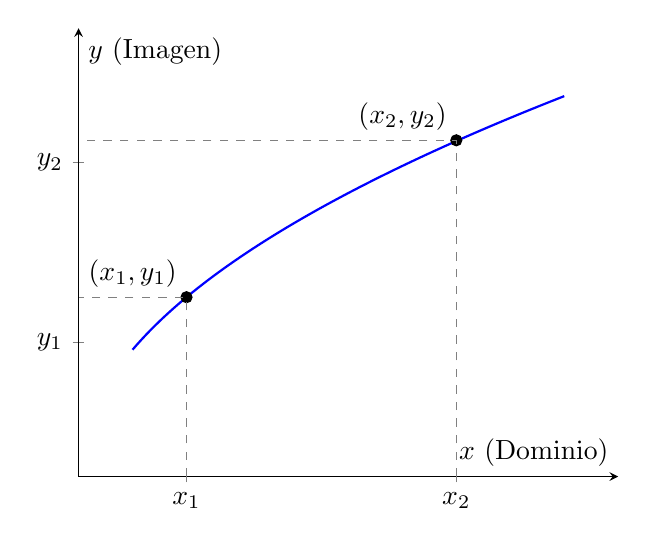
\begin{tikzpicture}
    \begin{axis}[
        axis lines = middle,
        xlabel = {$x$ (Dominio)},
        ylabel = {$y$ (Imagen)},
        xmin = 0, xmax = 5,
        ymin = 0, ymax = 4,
        xtick = {1, 3.5},
        xticklabels = {$x_1$, $x_2$},
        ytick = {1.2, 2.8},
        yticklabels = {$y_1$, $y_2$},
        grid = none,
        clip = false % Permite que las etiquetas no se corten
    ]
        % Dibujamos una curva suave en el primer cuadrante
        \addplot [domain=0.5:4.5, samples=100, thick, blue] {0.8*sqrt(x*4)};

        % Punto (x1, y1)
        \filldraw[black] (axis cs:1, 1.6) circle (2pt) 
            node[anchor=south east] {$(x_1, y_1)$};
        \draw [dashed, gray] (axis cs:1, 0) -- (axis cs:1, 1.6) -- (axis cs:0, 1.6);

        % Punto (x2, y2) con y0 
        % Aquí los pongo diferentes para ilustrar pares ordenados generales
        \filldraw[black] (axis cs:3.5, 3) circle (2pt) 
            node[anchor=south east] {$(x_2, y_2)$};
        \draw [dashed, gray] (axis cs:3.5, 0) -- (axis cs:3.5, 3) -- (axis cs:0, 3);

    \end{axis}
    \end{tikzpicture}
    \caption{visualización de \((x_1,y_1)\) y \((x_2,y_2)\)}
    \label{grafico_de_dominio_e_imagen}
\end{figure}


\begin{ejercicio}
\begin{enumerate}
  \item Dado \(S_1 = \{3,6,7\}, S_2 = \{a,b\}\) y \(S_3 = \{m.n\}\) determine los productos cartesianos: 
  
    \((a) S_1 \times S_2 = \quad\) Respuesta: \(\{(3,a),(6,a),(7,a),(3,b),(6,b),(7,b)\}\)
    
    \((b) S_2 \times S_3 = \quad\) Respuesta: \(\{(a,m),(a,n),(b,m),(b,n)\}\)
    
    \((c) S_3 \times S_1 = \quad\) Respuesta: \(\{(m,3),(m,6),(m,7),(n,3),(n,6),(n,7)\}\)     

  \item De la información del problema 1, encuentre el producto cartesiano \(S_1 \times S_2 \times S_3\).
  
  Respuesta: \(S_1 \times S_2 \times S_3 = \{(a,b,c) | a \in S_1 , b \in S_2 , c \in S_3\}\)
  \item En general, ¿Se cumple que \(S_1 \times S_2 = S_2 \times S_1\)? ¿En que condiciones estos dos productos cartesianos son iguales?
  
  Respuesta: No, no se cumple, ya que al ser pares ordenados el orden de cada elemento importa. Estos productos serian iguales si solo si \(S_1 = S_2\) o si uno de los dos es el conjunto vacío.
  \item ¿Por qué una recta con pediente descendente es una función y un rectangulo no?
  
  Porque la recta cumple las propiedades de unicidad y existencia. Por otro lado el rectangulo no cumple con la unicidad, por lo tanto no es una función. La unicidad corresponde a que a cada valor de \(x\) se le asigne un único valor \(y\).
  \item Si el dominio de la función \(y = 5 + 3x\) es el conjunto \(\{x |1 \leq x \leq 9\}\), determine la imagen de la función y expréselo como un conjunto.

  Respuesta: La imagen es \(\{y |8 \leq y \leq  32\}\)
  \item Para la función \(y = -x^2\), si el dominio es el conjunto de los números reales no negativos, ¿cuál es la imagen?
  
  Respuesta: Si el dominio son números positivos \((x≥0)\), al elevarlos al cuadrado dan positivo, pero el signo negativo de afuera los vuelve a todos negativos (o cero). La imagen es el conjunto de los números reales no positivos, es decir \(\mathbb{R}^-\) 
  \item En la teoría de la empresa, los economistas consideran el costo total \(C\) como una función del nivel de producción \(Q: C=f(Q)\).

  (a) De acuerdo con la definición de una función, ¿se debe relacionar cada cifra de costo con un nivel de producción único?

  Respuesta: La definición de función exige que para cada \(Q\) haya un solo \(C\), pero no obliga a que para cada \(C\) haya un solo \(Q\). Podría ser que producir \(10\) unidades cueste \(\mathdollar{100}\) y producir \(12\) unidades (por una gran eficiencia) también cueste \(\mathdollar{100}\). Eso sigue siendo una función. Lo que no puede pasar es que producir 10 unidades cueste \(\mathdollar{100}\) y \(\mathdollar{200}\) al mismo tiempo.

  (b) ¿Cada nivel de producción debe determinar una cifra de costo única?

  Respuesta: Si, a cada nivel de producción se le debe asignar solo una cifra de costo, esto para mantener la unicidad de la función. Es decir para una cantidad \(Q\) no puedo tener dos costos distintos.
  \item Si un nivel de producción \(Q_1\) se puede producir a un costo de \(C_1\), entonces también debe ser posible (por ser menos eficaz) producir \(Q_1\) a un costo de \(C_1 + \mathdollar{1}\), o \(C_1 + \mathdollar{2}\), etc. Así, parecería que el producto \(Q\) no sólo determina el costo total \(C\). Si así fuera, escribir \(C = f(Q)\) violaría la definición de una función. ¿Cómo, a pesar de este razonamiento, justificaría el uso de la función \(C = f(Q)\)?
  
  Respuesta: Se justifica mediante el supuesto de eficiencia técnica. La función \(C=f(Q)\) representa la relación de costo mínimo. Aunque existen infinitos costos ineficientes para producir una cantidad, la teoría económica se interesa solo en el resultado óptimo, logrando así que a cada nivel de producción le corresponda un único valor de costo (el más bajo posible), cumpliendo con la definición de función.
\end{enumerate}
\end{ejercicio}




\subsection{Tipos de función}

Hay varios tipos específicos dea función, cada uno representa una regla de mapeo constante

\subsubsection{Funciones constantes}

Una función cuya imagen consiste sólo en un elemento. Como la función 
\[
y=f(x)=7
\]
Que también se puede expresar como \(y=7\) o \(f(x)=7\), cuyo valor no cambia sin importar el valor de \(x\). Esta función es una recta horizontal, tal como se ve en la figura \ref{Type_funcion_constante}. Esta funcion se aplica en modelos como el ingreso nacional, cuando la inversión \(I\) se determina de manera exógena, se podría tener una función de inversión de la forma \(I=\mathdollar{100}\)millones, o bien \(I=I_0\).

\begin{figure}[!ht]
    \centering
    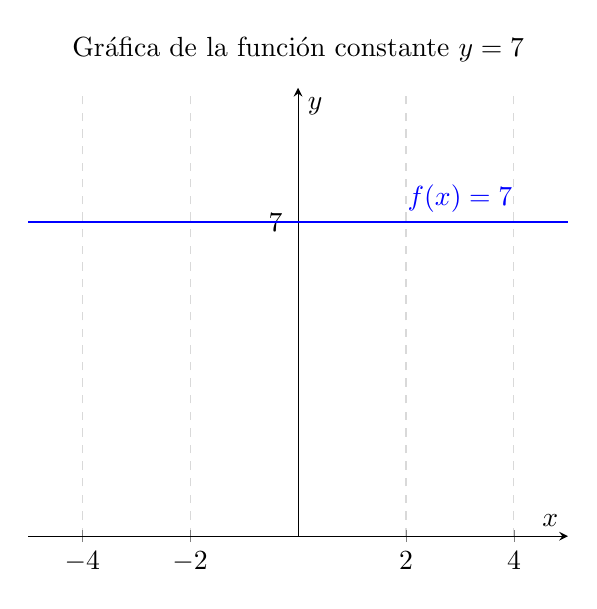
\begin{tikzpicture}
    \begin{axis}[
        axis lines = middle,                          % Ejes al centro (forma de cruz)
        xlabel = {$x$},                               % Etiqueta eje x
        ylabel = {$y$},                               % Etiqueta eje y
        ymin = 0, ymax = 10,                          % Rango visible en y
        xmin = -5, xmax = 5,                          % Rango visible en x
        ytick = {7},                                  % Marca específica en el 7
        grid = both,                                  % Mostrar cuadrícula
        grid style = {dashed, gray!30},
        title = {Gráfica de la función constante $y = 7$}
    ]
        % Dibujamos la función y = 7
        \addplot [
            domain=-5:5, 
            samples=2, 
            color=blue, 
            thick
        ] {7};

        % Añadimos un nodo para etiquetar la línea
        \node[above, blue] at (axis cs: 3, 7) {$f(x) = 7$};

    \end{axis}
    \end{tikzpicture}
    \caption{Función constante donde \(f(x)=7\)}
    \label{Type_funcion_constante}
\end{figure}



\subsubsection{Funciones polinomiales}

\textit{Polinomio} significa ``varios terminos'', una función polinomial se construye sumando diferentes ``piezas'' llamadas monomios. La razon por la que sumariamos los monomios es que cuando modelamos una realidad como la economía, se acumulan diferentes fuerzas o efectos, cada una de ellas es un monomio y el resultado de su combinación da el polinomio. Para entender esto bien, ver el ejemplo \ref{ejemplo_1.1.4}. Un polinomio tiene la forma general de 

\[
y=a_0+a_1x+a_2x^2+\dots+a_nx^n
\]

cada monomio contiene un coeficiente conocido\footnote{Las primeras letras del abecedario se usan como una forma de representar números conocidos en una ecuación.} \((a)\) y una potencia entera no negativa de la variable \(x\). Un polinomio puede tener valores de monomio \(0\), es decir puede ser que \(a_0 = 0, a_1x = 0\) y que \(a_2x^2 = n\) que nos daria una funcion cuadrática.

Dependiendo del valor del entero \(n\) (el cual especifica la mayor potencia de \(x\)), se tienen varias subclases de función polinomial:
\[
\begin{aligned}
\text{Caso de } n=0: & \quad y=a_0 && \text{[Función constante]} \\
\text{Caso de } n=1: & \quad y=a_0+a_1x && \text{[Función lineal]} \\
\text{Caso de } n=2: & \quad y=a_0+a_1x+a_2x^2 && \text{[Función cuadrática]} \\
\text{Caso de } n=3: & \quad y=a_0+a_1x+a_2x^2+a_3x^3 && \text{[Función cúbica]}
\end{aligned}
\]

Los superíndices de las potencias de \(x\) se llaman \textit{exponentes}. La mayor potencia que interviene, es decir el valor de \(n\), se denomina \textit{grado} de la función polinomial. En la función \(y = a_0+ a_1 + \dots +a_nx^n\) el orden de los monomios no tiene una relevancia, ya que esta dentro de una igualdad y conjunto de sumas. En vez de \(y\) se podria usar \(f(x)\).

En el caso de la función lineal (Figura \ref{type_funcion_lineal}) aparece como una recta. Cuando \(x=0\), la funcion lineal produce \(y=a_0\); así el par ordenado \((0,a_0)\) esta sobre la recta. Esto da la \textit{ordenada al origen} \(y\), porque es el punto donde el eje vertical se cruza con la recta. El otro coeficiente, \(a_1\), mide la \textit{pendiente} o el grado de inclinación de la recta. Un incremento unitario en \(x\) da como resultado un incremento en \(y\) en la cantidad de \(a_1\). Si \(a_1 > 0\) va a tener pendiente positiva, si \(a_1 < 0\) va a tener pendiente negativa o descendente.

\begin{figure}[htbp]
    \centering
    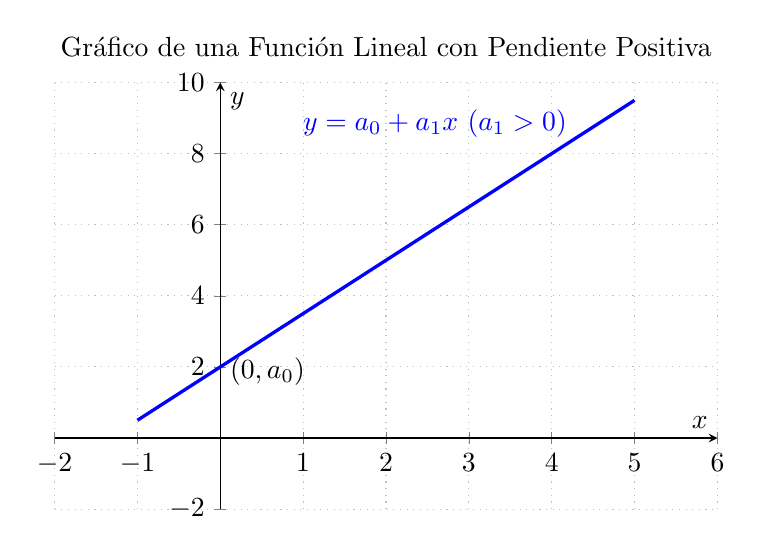
\begin{tikzpicture}
        \begin{axis}[
            axis lines = middle, % Ejes en el centro
            xlabel = $x$,
            ylabel = $y$,
            xmin=-2, xmax=6, % Rango del eje x
            ymin=-2, ymax=10, % Rango del eje y
            grid=major,
            major grid style={dotted},
            width=10cm, height=7cm,
            title={Gráfico de una Función Lineal con Pendiente Positiva},
        ]
        
        % Definimos la función f(x) = a0 + a1*x
        \addplot [
            domain=-1:5, % Rango de x para graficar la función
            samples=100,
            color=blue,
            very thick,
        ] {2 + 1.5*x};
        
        % Etiqueta para la ordenada al origen
        \node[anchor=south west] at (axis cs:0,1.2) {$(0, a_0)$};
        
        % Ecuación de la recta como etiqueta
        \node[anchor=north east, color=blue] at (axis cs:4.3, 9.5) {$y = a_0 + a_1x$ ($a_1 > 0$)};
        
        \end{axis}
    \end{tikzpicture}
    \caption{Gráfico de la función lineal con pendiente positiva.}
    \label{type_funcion_lineal}
\end{figure}

Una función cuadrática traza una parábola, como se ve en la figura \ref{type_funcion_cuadratica}. La función cúbica, muestra dos ondulaciones como se ve en la figura \ref{type_funcion_cubica}.

\begin{figure}[htbp]
    \begin{subfigure}[b]{0.48\textwidth}
        \centering
        \begin{tikzpicture}
            \begin{axis}[
                axis lines = middle, 
                xlabel = $x$, ylabel = $y$,
                xmin=-4, xmax=4, ymin=-1, ymax=10,
                grid = major, major grid style = {dotted},
                width=\textwidth, % Usa el ancho de la subfigura
                title={Cuadrática ($n=2$)}
            ]
            \addplot[domain=-3:3, samples=100, color=blue, very thick] {1 + x^2};
            \addplot[mark=*, only marks, color=black] coordinates {(0,1)};
            \end{axis}
        \end{tikzpicture}
        \caption{parábola con $a_2 > 0$}
        \label{type_funcion_cuadratica}
    \end{subfigure}
    \hfill
    \begin{subfigure}[b]{0.48\textwidth}
        \centering
        \begin{tikzpicture}
            \begin{axis}[
                axis lines = middle, 
                xlabel = $x$, ylabel = $y$,
                xmin=-3, xmax=3, ymin=-10, ymax=10,
                grid = major, major grid style = {dotted},
                width=\textwidth,
                title={Cúbica ($n=3$)}
            ]
            \addplot[domain=-2.2:2.2, samples=100, color=blue, very thick] {x^3 - 2*x + 1};
            \addplot[mark=*, only marks, color=black] coordinates {(0,1)};
            \end{axis}
        \end{tikzpicture}
        \caption{Función $y = x^3 - 2x + 1$}
        \label{type_funcion_cubica}
    \end{subfigure}
    \caption{Funciones polinomiales con exponente \(2\) y \(3\).}
    \label{funcion_cuadratica_y_cubica}
\end{figure}

\begin{ejemplo}
    \label{ejemplo_1.1.4}
    Imagina que quieres calcular el Costo Total \(C\) de producir palomitas en un cine. Ese costo se origina sumando diferentes monomios. El primer monomio seria el costo fijo supongamos \(\mathdollar100\) (Este incluye el alquiler de la maquina). El segundo monomio seria el costo variable lineal, supongamos que por cada balde de palomitas gastamos \(\mathdollar2\), entonces por cada balde vendido el costo sería \(2Q\) (donde \(Q\) es la cantidad). El tercer monomio seria costo de complejidad, donde a medida que producimos más, la maquina se calienta o necesita más personal, supongamos que incrementa el costo en \(\mathdollar0.05*2\) por cada incremento de complejidad, entonces nos quedaria \(0.05Q2\). 

    Al sumar los monomios obtenemos la función polinomial que seria \(C(Q)=0.05Q2+2Q+100\)
\end{ejemplo}



\subsubsection{Funciones racionales}

Una \textit{función racional} es aquella en la cual y se expresa como una razón de dos polinomios en la variable \(x\). Entonces una función racional es una proporción o una comparación entre dos polinomios, como por ejemplo
\[
y=x-1/x^2+2x+4
\]
Según su definición, cualquier función polinomial debe ser por sí misma una función racional, porque siempre se puede expresar como una razon respecto a 1, y 1 es una funcion constante.

Una función racional especial que tiene aplicaciones interesantes en la economía es la función
\[
y=a/x \qquad \text{o} \qquad xy=a
\]
Esta función describe una \textit{hipérbola rectangular} como en la figura \ref{type_funcion_racional}. Puesto que el producto de las dos variables es siempre una constante fija, esta funcion se puede usar para representar esa curva de demanda especial, con precio \(P\) y cantidad \(Q\) en los dos ejes, para la cual el gasto total \(PQ\) es constante en todos los niveles del precio. Otra aplicación es para el costo fijo promedio \((CFP)\), con \(CFP\) en un eje y el producto \(Q\) en el otro, la curva \(CFP\) debe ser hiperbólica rectangular porque \(CFP \times Q = Costo fijo total\).

\begin{figure}[htbp]
    \centering
    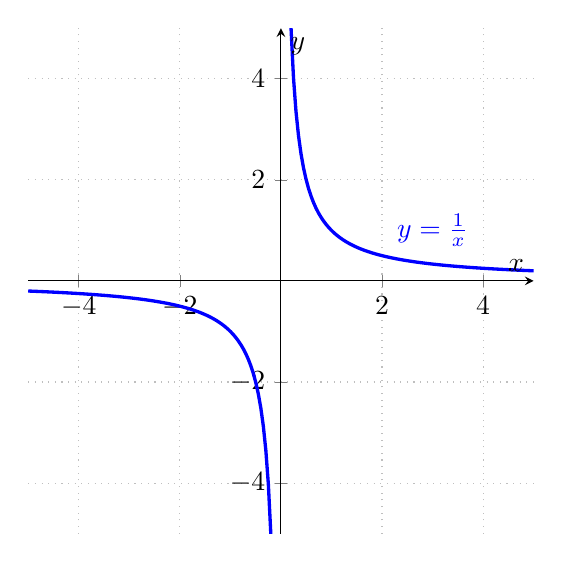
\begin{tikzpicture}
        \begin{axis}[
            axis lines = middle,
            xlabel = $x$,
            ylabel = $y$,
            xmin=-5, xmax=5,
            ymin=-5, ymax=5,
            grid = major,
            major grid style= {dotted},
            width=8cm, height=8cm,
        ]
        % Grafico y=1/x
        \addplot [
            domain=-5:-0.1,
            samples=100,
            color=blue,
            very thick,
        ] {1/x};
        \addplot [
            domain=0.1:5,
            samples=100,
            color=blue,
            very thick,
        ] {1/x};

        % Etiquetas
        \node[color=blue] at (axis cs:3, 1) {$y = \frac{1}{x}$};

        \end{axis}
    \end{tikzpicture}
    \caption{Gráfica de una hipérbola equilátera.}
    \label{type_funcion_racional}
\end{figure}

La hiperbola rectangular trazada a partir de \(xy=a\) nunca toca los ejes, incluso si se extiende de forma indefinida hacia arriba y a la derecha. Esta curva se aproxima \textit{asintóticamente} a los ejes: cuando \(y\) crece, la curba se aproxima cada vez mas al eje, pero nunca lo toca. Lo mismo ocurre con el eje \(x\), por eso se dice que los ejes constituyen las \textit{asíntotas}\footnote{Las asíntotas son rectas a las cuales la gráfica de una función se aproxima indefinidamente sin llegar a tocarlas o cruzarlas en el infinito.} de esta función.

Una asíntota es un ``muro invisible'' que tiene la funcion. La asíntota vertical, es el valor de \(x\) que hace que el denominador sea \(0\). Teniendo en cuenta el ejemplo \ref{ejemplo_1.1.5} si \(Q=0\), es decir nadie va al cine, el costo promedio es infinito. La gráfica se dispara hacia arriba intentando tocar el eje pero nunca lo logra.

En el caso de la asíntota horizontal, nos dice que pasa cuando los números se vuelven gigantes. Si vemos el ejemplo \ref{ejemplo_1.1.5}, si vendemos millones de entradas, los costos casi no importarian, y el costo promedio se ``estabilizaria'' cerca de \(2\).

\begin{ejemplo}
    \label{ejemplo_1.1.5}
    Imagina que quieres calcular el Costo Medio (lo que te cuesta cada entrada en promedio) de un cine. El polinomio de arriba \(P\) va a ser el costo total. Digamos \(C(Q)=2Q+100\). El polinomio de abajo \(Q\) va a ser la cantidad de personas que se estima que van a comprar entradas. Digamos simplemente \(Q\).
    Entonces la función racional resultante es 
    \[
    CMe(Q) = \frac{2Q + 100}{Q}
    \]
    Aquí, lo que estamos haciendo es ver cómo interactúan dos fuerzas. Arriba se encuentra el costo, y abajo el volumen de gente que reparte ese costo. Al dividirlos, conseguimos una información que ninguno de los polinomios podria dar por separado.
\end{ejemplo}

\begin{nota}
    En economía, las funciones racionales se usan siempre que se quiere hablar de promedios o de elasticidad.
\end{nota}


\subsubsection{Funciones no algebraicas}

Toda función expresada en términos de polinomios o raíces, o ambas cosas son \textit{funciones algebraicas}. Por lo tanto todas las funciones analizadas hasta aquí son funciones algebraicas.

Las \textit{funciones exponenciales} como \(y=b^x\), en la cual la variable independiente \((x)\) aparece en el exponente, son \textit{no algebraicas}. Otras funciones \textit{no algebraicas} son las logarítmicas y las trigonométricas. Las funciones no algebraicas tambien conocidas como \textit{funciones trascendetes} se estudiaran más adelante para que sea mas facil entender los conceptos.


\subsubsection{Digresión acerca de exponentes}

En fuciones polinomiales se introdujo el término \textit{exponente} como indicador de la potencia a la que está elevada una variable. Una potencia en general se define para un número entero positivo como
\[
x^n \equiv \underbrace{x \times x \times \dots \times x}_{n \text{ términos}}
\]
como caso especial, se da que \(x^1 = x\). De la definición general se deduce que para enteros positivos \(m\) y \(n\), los exponentes obedecen las siguientes reglas:

\textbf{Regla I}
\[
x^m \times x^m = x^{m+n} \qquad \text{Por ejemplo} x^3 \times x^4 = x^7
\]
Esto se demuestra o se puede comprobar de la siguiente manera
\[
x^m \times x^n = \underbrace{(x \times x \times \dots \times x)}_{m \text{ términos}} \underbrace{(x \times x \times \dots \times x)}_{n \text{ términos}}
\]
Por lo tanto 
\[
x^m \times x^n = \underbrace{(x \times x \times \dots \times x)}_{m+n \text{ términos}} = x^{m+n}
\]
En esta prueba no se asignó ningún valor específico al número \(x\), o a los exponentes \(m\) y \(n\). Así, el resultado obtenido es \textit{generalmente} cierto. Esta demostración constituye una prueba.

\textbf{Regla II}

\[
\frac{x^m}{x^n} = x^{m-n} \qquad \text{Por ejemplo} \frac{x^4}{x^3}=x
\]
Esto siempre que \(x \neq 0\). Esto se puede demostrar de la siguiente manera 
\[
\frac{x^m}{x^n} = \frac{\overbrace{(x \times x \times \dots \times x)}^{m \text{ términos}}}{\underbrace{(x \times x \times \dots \times x)}_{n \text{ términos}}} = \underbrace{(x \times x \times \dots \times x)}_{m-n \text{ términos}} = x^{m-n}
\]

Los términos del denominador y el numerador se cancelan. En caso de que \(x=0\) esta regla se descarta, ya que implicaria que hay una division entre \(0\), lo cual es indefinida.

Otro caso especial es si \(m=n\), que produce la expresion \(x^{m-n} = x^0\). Donde cualquier número elevado a la potencia \(0\) es igual a \(1\).

\textbf{Regla III}

Si en el caso de la regla anterior \(m<n\) nos da una potencia negativa de \(x\) como en el caso de que \(m=2\) y  \(n=5\), donde se tiene
\[
\frac{x^2}{x^5} = \frac{x \times x}{x \times x \times x \times x \times x} = \frac{1}{x \times x \times x} = \frac{1}{x^3} = x^{-3}
\]
Por lo tanto \(x^{-n}=\frac{1}{x^n}\) siempre que \(x \neq 0\). 

Elevar un número a una potencia negativa es tomar el recíproco de su \textit{n-ésima} potencia.

\textbf{Regla IV}

Otro caso especial de la regla dos es si \(m=n\), que produce la expresion \(x^{m-n} = x^0\). Donde cualquier número elevado a la potencia \(0\) es igual a \(1\). Es decir \(x^0=1\).

\textbf{Regla V}

En las funciones exponenciales, el exponente es una variable que puede tomar valores \textit{no enteros}. A fin de interpretar un número como \(x^{1/2}\), considerando la regla uno se tiene que 
\[x^{1/2} \times x^{1/2} = x^1 = x\]

Como \(x^{1/2}\) multiplicada por sí misma es \(x\), \(x^{1/2}\) es la raíz cuadrada de \(x\). 

Es decir que \[x^{1/n}=\sqrt[n]{x}\]

\textbf{Regla VI}
\[(x^m)^n = x^{mn}\]

\textbf{Regla VII} 
\[x^m \times y^m = (xy)^m\]

\begin{ejercicio}
    \begin{enumerate}
        \item Grafique las funciones 
        \[
        (a) \quad y = 16 + 2x \qquad (b) \quad y = 8 - 2x \qquad (c) \quad y = 12 + 2x
        \]
        Para cada caso considere que el dominio consiste sólo en los números reales no negativos.
        \item ¿Cuál es la diferencia principal entre \((a)\) y \((b)\) en el problema 1? ¿Cómo se refleja esta diferencia en las gráficas? ¿Cuál es la diferencia principal entre \((a)\) y \((c)\)? ¿Cómo la reflejan sus gráficas?
        \item Gráficas de funciones 
        \[
        (a) \quad y = -x^2 + 5x - 2 \qquad (b) \quad y = x^2 + 5x - 2
        \]
        Con el conjunto de valores \(-5 \leq x \leq 5\) que constituye el dominio. Es sabido que el signo del coeficiente del término \(x^2\) determina si la función cuadrática tiene una ``colina'' o un ``valle''. Con base en el presente problema ¿Qué signo se relaciona con la colina? proporcione una explicación.
        \item Grafique la función \(y = 36/x\), suponiendo que \(x\) y \(y\) pueden tomar valores positivos solamente. A continuación, suponga que ambas variables pueden tomar valores negativos también; ¿Cómo se debe modificar la grafica para reflejar ese cambio?
        \item Condense las expresiones siguientes: 
        \[
        (a) \quad x^4 \times x^{15} \qquad (b) \quad x^a \times x^b \times x^c \qquad (c) \quad x^3 \times y^3 \times z^3
        \]
        \item Determine: \((a) x^3/x^{-3} \qquad \frac{(b)x^{1/2} \times x^{1/3}}{x^{2/3}}\)
        \item Demuestre que \(x^{m/n}=\sqrt[n]{x^m}=(\sqrt[n]{x})^m\). Especifque las reglas aplicadas en cada paso.
    \end{enumerate}

    \textit{Respuestas}

    \begin{enumerate}
        \item Ver figura \ref{grafico_ejercicios_1.1.x_a}

        \item La diferencia principal radica en los valores y los signos de los monomios, \(a\) tiene su ordenada en \(16\) y su pendiente \(2x\) es positiva, mientras que \(b\) tiene su origen en \(8\) y tiene una pendiente \(-2x\) negativa. Esto en las gráficas es facil de diferenciar por las pendientes. 
        
        La diferencia entre \(a\) y \(c\) se encuentra en la ordenada de origen, ya que su pendiente es la misma \((2x)\), en \(a\) la ordenada es \(16\) y en \(c\) la ordenada es \(12\). Esto se ve en el punto donde \(x\) intersecta con el eje \(y\).
        \item Ver figura \ref{grafico_ejercicios_1.1.x_b}. El signo que relaciona que sea una ``colina'' o un ``valle'' es el de \(x^2\), cuando este es negativo se forma una colina, mientras que si este es positivo se forma un valle. 
        \item Ver figura \ref{grafico_ejercicios_1.1.x_c}. En la grafica si tomamos valores negativos vamos a ver una forma similar a la del positivo pero en ves de que esté en el primer cuadrante, está va a estar en el tercer cuadrante.
        \item \((a) = x^{19} \qquad (b) = x^{a+b+c} \qquad (c)= (xyz)^3\)
        \item \((a) = x^6 \qquad (b)=\frac{x^{5/6}}{x^{2/3}}= x^{1/6}\)
        \item \(x^{m/n} = \sqrt[n]{x^m}\) ya que siguiendo la regla V \(x^{1/n} = \sqrt[n]{x} \implies x^{m/n}= \sqrt[n]{x^m}\). En el caso del otro siguiendo con la regla V \(x^{m/n}=(\sqrt[n]{x})^m\), ya que \(\sqrt[n]{x^1} = x^{1/n} \implies (\sqrt[n]{x})^m\).
    \end{enumerate}
\end{ejercicio}

% --------------------------- %
% GRAFICA DE LINEAL EJERCICIO %
% --------------------------- %

\begin{figure}[htbp]
    \centering 
    % --- Primera fila: Gráficas (a) y (b) ---
    \begin{subfigure}[b]{0.45\textwidth}
        \centering
        \begin{tikzpicture}
            \begin{axis}[
                axis lines = middle, xlabel = $x$, ylabel = $y$,
                xmin=0, xmax=4, ymin=0, ymax=25, % Ajustado a dominio no negativo
                grid = major, major grid style = {dotted}, width=\textwidth,
                title={$y=16+2x$}
            ]
            \addplot[domain=0:4, samples=50, color=blue, very thick] {16+2*x};
            \end{axis}
        \end{tikzpicture}
        \caption{Función (a)}
    \end{subfigure}
    \hfill % Espacio máximo entre las dos figuras de arriba
    \begin{subfigure}[b]{0.45\textwidth}
        \centering
        \begin{tikzpicture}
            \begin{axis}[
                axis lines = middle, xlabel = $x$, ylabel = $y$,
                xmin=0, xmax=4, ymin=0, ymax=10,
                grid = major, major grid style = {dotted}, width=\textwidth,
                title={$y=8-2x$}
            ]
            \addplot[domain=0:4, samples=50, color=blue, very thick] {8-2*x};
            \end{axis}
        \end{tikzpicture}
        \caption{Función (b)}
    \end{subfigure}

    \vspace{0.5cm} % Espacio vertical entre las filas

    % --- Segunda fila: Gráfica (c) centrada ---
    \begin{subfigure}[b]{0.45\textwidth}
        \centering
        \begin{tikzpicture}
            \begin{axis}[
                axis lines = middle, xlabel = $x$, ylabel = $y$,
                xmin=0, xmax=4, ymin=0, ymax=25,
                grid = major, major grid style = {dotted}, width=\textwidth,
                title={$y=12+2x$}
            ]
            \addplot[domain=0:4, samples=50, color=blue, very thick] {12+2*x};
            \end{axis}
        \end{tikzpicture}
        \caption{Función (c)}
    \end{subfigure}

    \caption{Gráficos de las funciones lineales del ejercicio 1.}
    \label{grafico_ejercicios_1.1.x_a}
\end{figure}

% ------------------------------- %
% GRAFICA DE POLINOMICA EJERCICIO %
% ------------------------------- %

\begin{figure}[htbp]
    \centering 
    % --- Primera fila: Gráficas (a) y (b) ---
    \begin{subfigure}[b]{0.45\textwidth}
        \centering
        \begin{tikzpicture}
            \begin{axis}[
                axis lines = middle, xlabel = $x$, ylabel = $y$,
                xmin=-1, xmax=5, ymin=-5, ymax=5,
                grid = major, major grid style = {dotted}, width=\textwidth,
                title={$y=-x^2+5x-2$}
            ]
            \addplot[domain=-5:5, samples=50, color=blue, very thick] {-x^2+5*x-2};
            \end{axis}
        \end{tikzpicture}
        \caption{Función (a)}
    \end{subfigure}
    \hfill % Espacio máximo entre las dos figuras de arriba
    \begin{subfigure}[b]{0.45\textwidth}
        \centering
        \begin{tikzpicture}
            \begin{axis}[
                axis lines = middle, xlabel = $x$, ylabel = $y$,
                xmin=-5, xmax=1, ymin=-9, ymax=1,
                grid = major, major grid style = {dotted}, width=\textwidth,
                title={$y=x^2+5x-2$}
            ]
            \addplot[domain=-5:5, samples=50, color=blue, very thick] {x^2+5*x-2};
            \end{axis}
        \end{tikzpicture}
        \caption{Función (b)}
    \end{subfigure}

    \caption{Gráficos de las funciones polinómicas del ejercicio 3.}
    \label{grafico_ejercicios_1.1.x_b}
\end{figure}

% ----------------------------- %
% GRAFICA DE RACIONAL EJERCICIO %
% ----------------------------- %

\begin{figure}[htbp]
    \centering 
    % --- Gráfica (a) ---
    \begin{subfigure}[b]{0.48\textwidth}
        \centering
        \begin{tikzpicture}
            \begin{axis}[
                axis lines = middle, xlabel = $x$, ylabel = $y$,
                xmin=0, xmax=12, ymin=0, ymax=45,
                grid = major, major grid style = {dotted}, width=\textwidth, 
                title={$y=36/x$ con valores positivos}
            ]
            \addplot[domain=0.8:12, samples=50, color=blue, thick] {36/x};
            \end{axis}
        \end{tikzpicture}
    \end{subfigure}
    \hfill 
    \begin{subfigure}[b]{0.48\textwidth}
        \centering
        \begin{tikzpicture}
            \begin{axis}[
                axis lines = middle, xlabel = $x$, ylabel = $y$,
                xmin=-12, xmax=2, ymin=-45, ymax=10,
                grid = major, major grid style = {dotted}, width=\textwidth,
                title={$y=36/x$ con valores negativos}
            ]
            \addplot[domain=-12:-0.8, samples=50, color=blue, thick] {36/x};
            \end{axis}
        \end{tikzpicture}
    \end{subfigure}

    \caption{Representación de la hipérbola $y = 36/x$.}
    \label{grafico_ejercicios_1.1.x_c}
\end{figure}



\clearpage
\subsection{Funciones de dos o más variables independientes}

Una función puede tener dos o más variables independientes. Una función de una variable independiente es \(y=f(x)\), una función de dos variables independientes es
\[
z=g(x,y)
\]
Un determinado par de valores \(x,y\) determina de manera única un valor de la variable dependiente \(z\). Es decir que \(z\) es igual a 
\[
z=ax+by \qquad \text{o} \qquad z = a_0+a_1x+a_2x^2+b_1y+ b_2y^2
\]

Al igual que la función \(y=f(x)\) que mapea un \textit{dominio} hacia un punto en la \textit{imagen}, la función \(g\) hace lo mismo. Sin embargo, en este caso el dominio no es un conjunto de números, es un conjunto de \textit{pares ordenados} \(x,y\), ya que se puede determinar \(z\) cuando se especifica \(x,y\).
La función g es un mapeo de un punto en un espacio bidimensional hacia un punto en un segmento de recta (es decir, un punto en un espacio unidimensional), por ejemplo del punto \(x_1, y_1\) hacia el punto \(z_1\) o de \(x_2, y_2\) hacia \(z_2\) como en la figura \ref{grafico_tidimensional_1}.

% \begin{figure}[htbp] % Realizar figura tridimensional 2.9a página 47
%     a
% \end{figure}

Si se coloca al eje \(z\) de forma perpendicular vertical al plano \(xy\), como se hizo en la figura \ref{grafico_tridimensional_2}, se obtiene un espacio tridimensional en la cual se le da a la función \(g\) una grafica más aproximada.
El dominio de esta función es algún subconjunto de los puntos en el plano \(xy\), y el valor de la función (valor \(z\)) para un punto en el dominio, se puede indicar mediante la altura de una recta vertical.
La relación de las tres variables se resume por una terna ordenada \(x_1,y_1,z_1\), que es el punto específico en el espacio tridimensional.
El lugar de esa terna ordenada es la que da forma a una superficie, que constituye la gráfica de la función \(g\).

\begin{nota}
    En economía se utiliza frecuentemente este tipo de funciones tridimensionales. Por ejemplo en las funciones de producción. Donde la producción se determina mediantes cantidades de capital \(k\), y la mano de obra empleada \(L\). Entonces se puede escribir una función de producción como \(Q=Q(K,L)\).
\end{nota}

Se pueden abarcar tres o más variables independientes. Una función como \(y=h(u,v,w)\), se puede mapear un punto del espacio tridimensional \((u_1, v_1, w_1)\), hacia un punto en un espacio unidimensional \((y_1)\). Está función podria indicar la utilidad del consumidor en relación a su consumo (en este caso de tres artículos).
La limitación se encuentra en su grafica, hasta ahora no hay un metdo para graficar una funcion de más de tres dimensiones.
La relación de estas ternas ordenadas, dan un punto en un espacio de más de tres dimensiones, estos puntos aunque no sea posible para el humano realizar, genera una gráfica, a esta gráfica se le llama \textit{hipersuperficie}.

Las funciones de más de una variable se clasifícan en varios tipos. Por ejemplo una función 
\[
y=a_1x_1+a_2x_2+\dots+a_nx_n
\]
es una función lineal, donde su caracterísitica es que cada variable es elevada sólo a la primera potencia.
Una función cuadrática, tiene que ver con primeras y segundas potencias de una o más variables independientes, pero la suma de los exponentes de las variables que aparecen en cualquier término simple no debe pasar de 2.

\begin{nota}
    En lugar de denotar las variables independientes mediante \(x,u,v,w, \dots\), se intercambiaron por \(x_{subíndice}\), es decir \(x_1,_x_2, \dots, x_n\).
    Este metodo, es una forma en econoía de contear más facil un mayor número de variables que forman parte de la función.
\end{nota}

\subsection{Niveles de generalidad}

En el análisis económico hay tres niveles de abstracción. El \textit{numérico} que es aquel donde las funciones con coeficientes fijos como \(y=6x+1\) ofrecen soluciones exactas, pero carecen de flexibilidad ante cambios.
El \textit{paramétrico} es aquel donde el uso de constantes simbólicas \(y=a+bx\) permite crear ``familias de curvas'' y obtener soluciones generales que no requieren repetir todo el procedimiento lógico si los datos cambian.
Y por ultimo el \textit{nivel general}, que alcanza la máxima aplicabilidad teórica al no restringirse a una forma geométrica específica como \(y=f(x)\). El ultimo sirve de forma económica para saber el comportamiento de la variable, por ejemplo en el caso de la demanda una forma general de describirla seria \(Q=f(p)\) al cual \(f(p)<0\), lo que quiere decir que tiene una pendiente negativa y que anate una subida del precio baja la demanda. Es la regla de comportamiento de la función. Mientras que la numérica y la paramétrica son para resolver una función ya sea de forma general o específica.

